\documentclass[russian,utf8,nocolumnxxxi,nocolumnxxxii]{eskdtext}
\usepackage[T1,T2A]{fontenc}
\usepackage[utf8]{inputenc}
\usepackage{amssymb,amsmath}
\usepackage{float}
\usepackage{tikz}
\usepackage{rotating}
\usepackage{graphicx}
\graphicspath{{pictures/}}
\DeclareGraphicsExtensions{.pdf,.png,.jpg}
\usepackage{pgfplots}
\usepackage{lipsum}
\usepackage{nccmath}
\usepackage{xcolor}
\usepackage{hyperref}
\definecolor{linkcolor}{HTML}{799B03} % цвет ссылок
\definecolor{urlcolor}{HTML}{799B03} % цвет гиперссылок
\hypersetup{pdfstartview=FitH,  linkcolor=linkcolor,urlcolor=urlcolor, colorlinks=true}
\usepackage{siunitx}
\usepackage[european,cuteinductors,smartlabels]{circuitikz}
\usepackage[backend=biber]{biblatex}

\begin{document}

\bf{\centering Федеральное агенство по образованию
САНКТ-ПЕТЕРБУРГСКИЙ ГОСУДАРСТВЕННЫЙ
ЭЛЕКТРОТЕХНИЧЕСКИЙ УНИВЕРСИТЕТ 
«ЛЭТИ» ИМ. В.И. УЛЬЯНОВА (ЛЕНИНА)\\[4cm]


Пояснительная записка к Курсовой работе\\[0.2cm]
по дисциплине «Информатика»\\[0.6cm]
Вариант 14\\[6cm]

Студент гр. 8871 \hspace{4cm}		Лоскутов Д.А.\\[0.4cm]
Преподаватель \hspace{4cm}		Прокшин А.Н.\\[1.5cm]


Санкт-Петербург\\[0.3cm]
2019\\}


\newpage

\\{\bfСодержание}
\\\ref{1}. Цель и тема курсовой работы \hspace{9cm} 3
\\\ref{2}. Задание на курсовую работу \hspace{9.5cm} 4
\\\ref{3}. Введение \hspace{14.5cm} 5 
\\\ref{4}. Исследование функции \hspace{11cm} 6
\\\ref{5}. Исследование кубического сплайна \hspace{8cm}13
\\\ref{6}. Задача оптимального распределения неоднородных ресурсов \hspace{1cm} 19
\\\ref{7}. Выводы \hspace{14.5cm} 23
\\\ref{8}. Список литературы \hspace{11.5cm} 24\\[14cm]
ссылка на сайт \href{https://github.com/DizZzelll}{https://github.com/DizZzelll}
\newpage
\begin{equation}\label{1}
\end{equation}
 {\large\bf 1. Цель и тема курсовой работы}

\\{\bf{Целью курсовой работы:}} является применение навыков использования ПЭВМ и математических пакетов прикладных программ в инженерной деятельности.
\\{\bfТема курсовой работы:} решение математических задач с использованием математического пакета «SciLab» и системы компьютерной алгебры «Reduce».

\newpage

\begin{equation}\label{2}
\end{equation}
{\large\bf2. Задания на курсовую работу}
\\1. Даны функции $f(x)=\sqrt{3}sin(x)+cos(x),g(x)=cos(2x+\frac{\pi}{3})-1$
\\а)Решить уравнение f(x)=g(x).
\\б)Исследовать функцию h(x)=f(x)-g(x) на промежутке $[0;\frac{5\pi}{6}]$
\\2. Найти коэффициенты кубического сплайна, интерполирующего данные, представленные в векторах:\\
$V_{x}=[0,0.75,1.6,2.375,3.75]$
$V_{y}=[5,4.8,5.7,5.5,5.0]$\\
Построить на графике функции f(x),полученную после нахождения коэффициентов кубического сплайна. \\
Представить графическое изображение результатов интерполяции исходных данных различными методами с использованием встроенных функций splin(x,y,“natural”), splin(x,y,“clamped”), splin(x,y,“not\_a\_knot”), splin(x,y, “fast”), splin(x,y,“monotone”), interp(xx,x,y,d)\\
3. Решить задачу оптимального распределения неоднородных ресурсов.
Требуется решить следующую задачу оптимального распределения неоднородных ресурсов. Пусть в распоряжении завода железобетонных изделий (ЖБИ) имеется m видов сырья (песок, щебень, цемент) в объемах ${\bf a_i}$  .Требуется произвести продукцию {\bf n} видов. Дана технологическая норма $c_ij$  требления отдельного i-го вида сырь для изготовления единицы продукции каждого j-го вида. Известна прибыль $\pi_j$  получаема от выпуска единицы продукции j-го вида. Требуется определить, какую продукцию и в каком количестве должен производить завод ЖБИ, чтобы получить максимальную прибыль.

\begin{figure}[H]
\begin{center}
\begin{minipage}[h]{0.5\linewidth}
\center{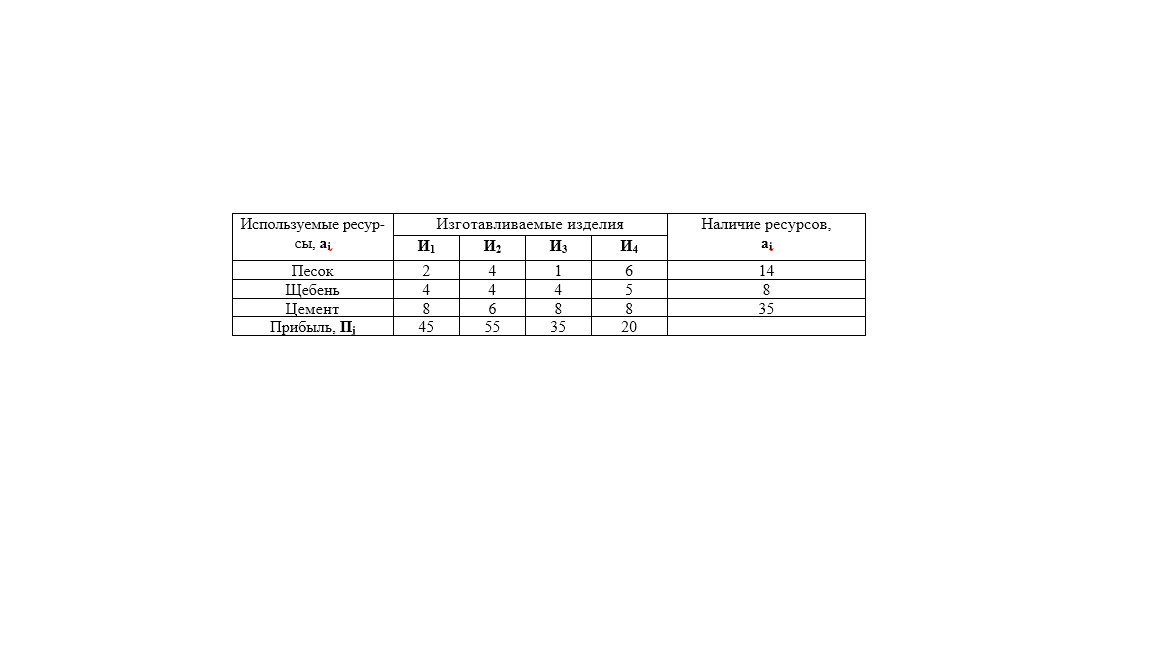
\includegraphics[width=0.8\linewidth]{1.png}}  \\
\end{minipage}
\end{center}
\end{figure}

\newpage
\begin{equation}\label{3}
\end{equation}

{\bf3. Введение:} Использование пакетов прикладных программ на ПВЭМ позволяет решать различные математические задачи, имеющий ярко выраженный прикладной характер
\newpage
\begin{equation}\label{4}
\end{equation}
{\bf4. Исследование функции}
\\Задание: 1. Даны функции
\\$f(x)=\sqrt{3}sin(x)+cos(x)$

\begin{figure}[H]
\begin{center}
\begin{minipage}[h]{0.65\linewidth}
\center{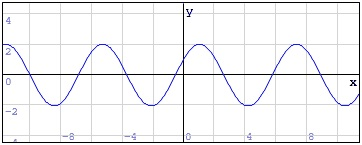
\includegraphics[width=1\linewidth]{2.jpg}}  \\
\end{minipage}
\end{center}
\end{figure}

\\$g(x)=cos(2x+\frac{\pi}{3})-1$

\begin{figure}[H]
\begin{center}
\begin{minipage}[h]{0.65\linewidth}
\center{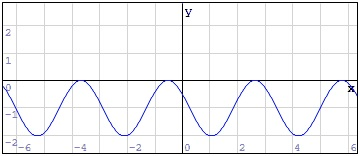
\includegraphics[width=1\linewidth]{3.jpg}}  \\
\end{minipage}
\end{center}
\end{figure}

\\а)Решить уравнение f(x)=g(x).
\\б)Исследовать функцию h(x)=f(x)-g(x) на промежутке $[0;\frac{5\pi}{6}]$\\
{\bfРешение уравнения.}\\
в) найти корни уравнения:\\
$h(x)=\sqrt{3}sin(x)+cos(x)-cos(2x+\frac{\pi}{3})-1$\\
\newpage
{\bfРешение задачи (а)}
Рассмотрим функцию f(x) и g(x):\\

\begin{figure}[H]
\begin{center}
\begin{minipage}[h]{0.65\linewidth}
\center{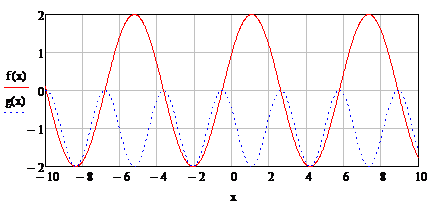
\includegraphics[width=1\linewidth]{132.png}}  \\
\end{minipage}
\end{center}
\end{figure}

Решим уравнение $f(x)=g(x)$ преобразуя выражение в вид $f(x)-g(x)=0$, а также применив упрощенную формулу $cos2x=1-2sin^2x$ и $sin(x+y)=sin(x)cos(y)+sin(y)cos(x)$ :\\

$\sqrt{3}*sin(x)+cos(x)=cos(2*x+\pi/3)-1$\\
$\sqrt{3}*sin(x)+cos(x)-cos(2*x+\pi/3)+1=0$\\
$2(sin(x)cos(\pi/6)+cos(x)sin(\pi/6)-(1-2sin^2(x+\pi/6)+1=0$\\
$2sin(x+\pi/6)+2sin^2(x+\pi/6)=0$\\
$2sin(x+\pi/6)*(1+sin(x+\pi/6)=0$\\

Применим к нему из мат.пакета "Reduce" функцию solve: \\



\begin{figure}[H]
\begin{center}
\begin{minipage}[h]{0.65\linewidth}
\center{\includegraphics[width=1\linewidth]{25.png}}  \\
\frametitle{}
\end{minipage}
\end{center}
\end{figure}


где arbint - произвольное целое число. Запишем решение в форме:

$$x_1=\frac{5}{6}*\pi+2n\pi,n\in Z$$
$$x_2=-\frac{1}{6}*\pi+2n\pi,n\in Z$$
$$x_3=\frac{8}{6}*\pi+2n\pi,n\in Z$$
$$x_4=-\frac{4}{6}*\pi+2n\pi,n\in Z$$\\
Периодические решения для $x_3$ и $x_4$ совпадают (возьмем любое), периодическое решение для $x_2$ запишем в виде:
$$x_2=\frac{11}{6}*\pi+2n\pi,n\in Z$$\\


\newpage
б)Исследуем функцию h(x)=f(x)-g(x) на промежутке $[0;\frac{5\pi}{6}]$\\
При решении нелинейных уравнений в «SciLab» с помощью стандартных функций получаем только численные решения, для нахождения аналитического будем использовать систему компьютерной алгебры «Reduce».\\
{\bfОтыскание численного решения.}\\
Для нахождения численного решения воспользуемся стандартной функцией «SciLab» fsolve.\\
Для отыскания начальных точек построим график функции h(x):\\
function y=h(x)\\
y=sqrt(3)*sin(x)+cos(x)-cos(2*x+\%pi/3)+1\\
endfunction\\
plot(0:0.01:2*pi,h)\\

\begin{figure}[H]
\begin{center}
\begin{minipage}[h]{0.65\linewidth}
\center{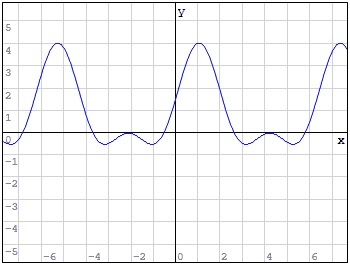
\includegraphics[width=1\linewidth]{4.jpg}}  \\
\end{minipage}
\end{center}
\end{figure}

\newpage
График периодичен, рассмотрим участок [0:5pi/6] :

\begin{figure}[H]
\begin{center}
\begin{minipage}[h]{0.65\linewidth}
\center{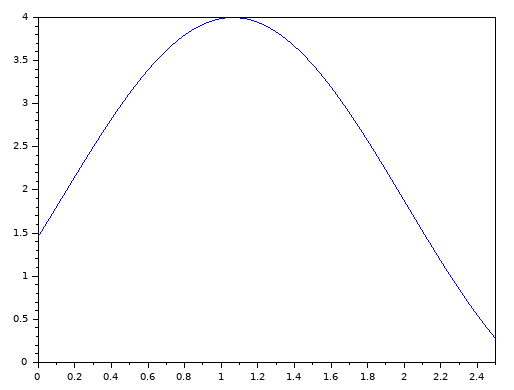
\includegraphics[width=1\linewidth]{134.png}}  \\
\end{minipage}
\end{center}
\end{figure}

Найдём производную функции h(x) :\\
Для этого воспользуемся мат.пакетом Maple, которое позволит найти производную практически любой функции.\\

\begin{figure}[H]
\begin{center}
\begin{minipage}[h]{0.65\linewidth}
\center{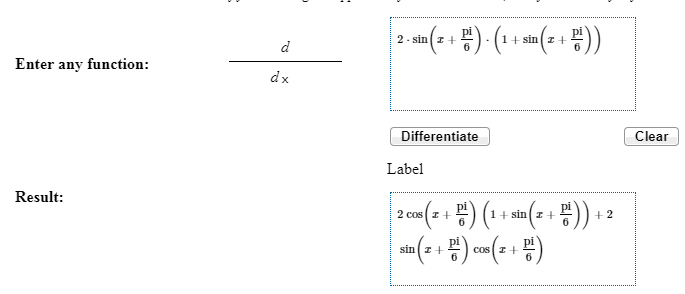
\includegraphics[width=1\linewidth]{135.png}}  \\
\end{minipage}
\end{center}
\end{figure}

Найдем точки, которые лежат в диапазоне от [0:5*pi/6]\\

\begin{figure}[H]
\begin{center}
\begin{minipage}[h]{0.65\linewidth}
\center{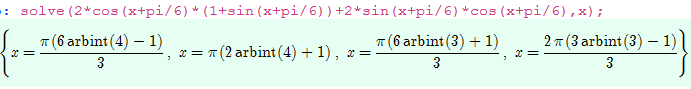
\includegraphics[width=1\linewidth]{136.png}}  \\
\end{minipage}
\end{center}
\end{figure}
\newpage

Как можем заменить, только одно значение x нам подходит, это x=pi/3 (функция h(x) при x=pi/6 > 0, а x=pi/2 < 0, следовательно x=pi/3 точка максимума) \\
подставим значение x в уравнение h(x) :

\begin{figure}[H]
\begin{center}
\begin{minipage}[h]{0.65\linewidth}
\center{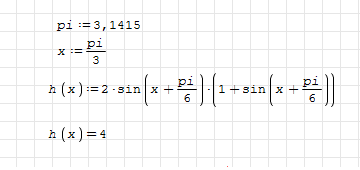
\includegraphics[width=1\linewidth]{137.png}}  \\
\end{minipage}
\end{center}
\end{figure}

Рассмотрим значения функции на концах отрезка [0:5*pi/6]:

\begin{figure}[H]
\begin{center}
\begin{minipage}[h]{0.65\linewidth}
\center{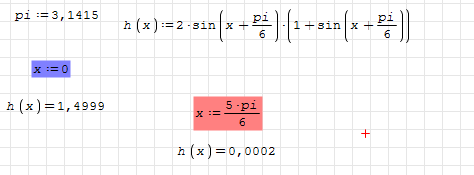
\includegraphics[width=1\linewidth]{138.png}}  \\
\end{minipage}
\end{center}
\end{figure}

Где x=3/2 - точка глобального максимума, а x=0 - точка глобального минимума. \\

найдём 2 производную h(x):\\
$-2*sin(x+pi/6)*(1+sin(x+pi/6)+2*cos(x+pi/6)*2*cos(x+pi/6)$\\
$-2*cos^2(x+pi/6)-2*sin^2(x+pi/6)-2*sin(x+pi/6)$\\
$2-2*sin^2(x+pi/6)-2*sin^2(x+pi/6)-2*sin(x+pi/6)$\\
$2-4*sin^2(x+pi/6)-2*sin(x+pi/6)=0$\\
\newpage
решим квадратное уравнение:\\
$2-4a^2-2a=0$\\
$2a^2+a-1=0$\\
$a1=-1$\\
$a2=1/2$\\
a)\\
$sin(x+pi/6)=-1$\\
$x+pi/6=-pi/2+2piK$\\
$x=-2*pi/3+2piK$\\
$x=4*pi/3$- не лежит на отрезке [0:5pi/6]\\

б)
$sin(x+pi/6)=1/2$
$x+pi/6=pi/6+pk$
$x=2piK$-получается значения x=2pi/3 и х=0,но х=0, это не внутренняя точка

Следовательно точка перегиба функции х=2pi/3\\

1) Возрастает на (0,$\frac{\pi}{3}$)

2) Убывает на ($\frac{\pi}{3},5\frac{\pi}{6}$)

3) Имеет глобальный максимум в точке $x=0$

4) Имеет глобальный минимум в точке $x=5\frac{\pi}{6}$

5) Точки перегиба x=2pi/3

6) Выпукла вверх при $0,\frac{2*\pi}{3}$)

7) Выпукла вниз при $\frac{2*\pi}{3},(5*\pi)/6$)

\newpage
\begin{equation}\label{5}
\end{equation}
\begin{center}{\bf5. Исследование кубического сплайна.}\end{center}
\par
\normalsize Найти коэффициенты кубического сплайна, интерполирующего данные, представленные в векторах:\\
$V_{x}=[0,0.75,1.6,2.375,3.75]$
$V_{y}=[5,4.8,5.7,5.5,5]$\\
Построить на графике функции f(x),полученную после нахождения коэффициентов кубического сплайна. 
\\Оценить погрешность интерполяции в точке x=2.4 Вычислить значение функции в точке x=1.4
\\Представить графическое изображение результатов интерполяции исходных данных.
\newpage
\begin{center}{\bf Нахождение коэффициентов кубического сплайна.}\\\end{center}
\par
\normalsize
Найдем уравнение сплайна проходящего через пять точкек $(x_{1}, y_{1}),\\
(x_{2}, y_{2}), (x_{3}, y_{3}) и (x_{4}, y_{4}) и (x_{5}, y_{5})$. Для того чтобы потенциальная энергия изогнутой
металлической линейки(сплайна) принимала минимальное значение,
производная четвертого порядка должна быть равна нулю, представим сплайн полиномом третьей степени на каждом отрезке
$[x_i, x_{i+1}]$
\\$$F_i(x) = A_{i0} + A_{i1}x + A_{i2}x^2 + A_{i3}x^3, где x \in [x_i, x_{i+1}]$$
Найдем коэффициэнты Aij исходя и того, что в точках склейки функция
не имеет разрывов, изломов и изгиб ее слева и справа совпадает. На каждом
из отрезков [xi, xi+1] график Fi(x) проходит через точки yi, yi+1 или
Fi(xi) = yi, Fi(xi+1) = yi+1. Записывая равенства через коэффициэнты Aij :
$yi = Ai0 + Ai1xi + Ai2x2i + Ai3x3i$
\par
\normalsize Составляем 8 уравнений, два на каждый участок кривой.
\begin{center}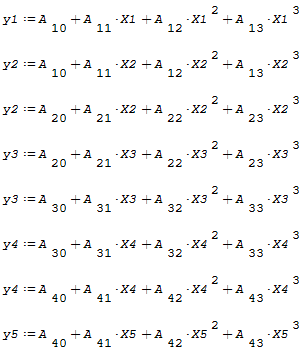
\includegraphics[scale=0.8]{11.png}\end{center}
\par
\newpage
\normalsize
При избежании излома сплайна, добавляем три уравнения с производными первого порядка.
\begin{center}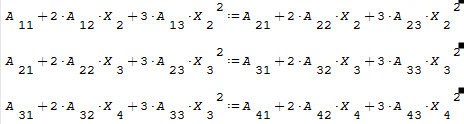
\includegraphics[scale=0.8]{12.png}\end{center}
\par
\normalsize
Для получения изгиба с каждой стороны добавляем три уравнения с производными второго порядка.
\begin{center}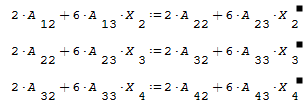
\includegraphics[scale=0.8]{13.png}\end{center}
\par
\normalsize
Уравнения отвечающие за положение концов сплайна представленны свободно.
\begin{center}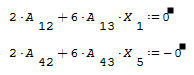
\includegraphics[scale=0.8]{14.png}\end{center}
\newpage
\par
\normalsize
Найденые 16 уравнений составляют матрицу размерностью 16х16. Находим коофициенты кубического сплайна.
\begin{center}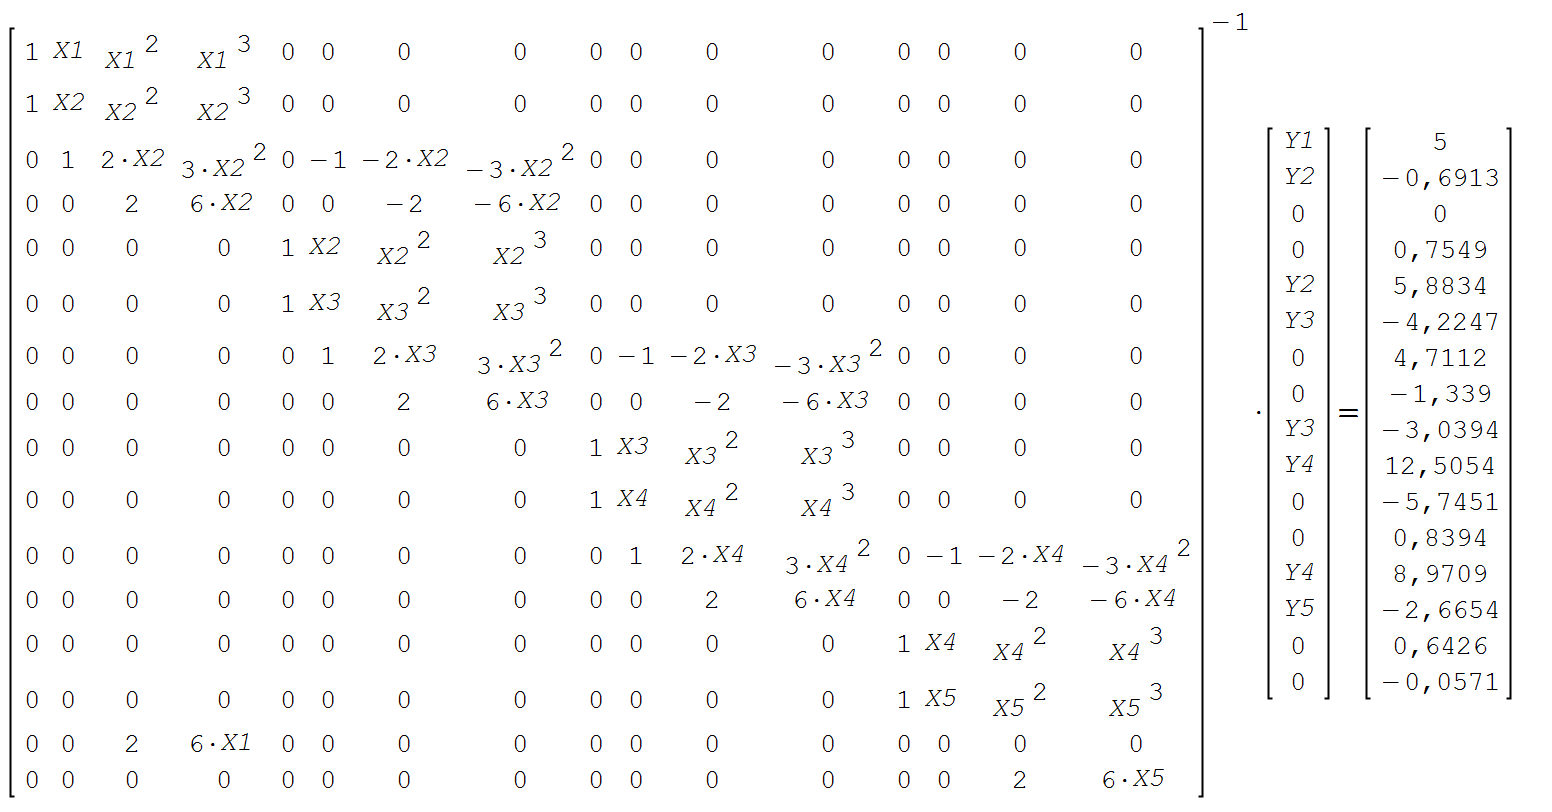
\includegraphics[scale=0.4]{15.png}\end{center}

\par
\normalsize
Конечное уравнение сплайна.
\begin{center}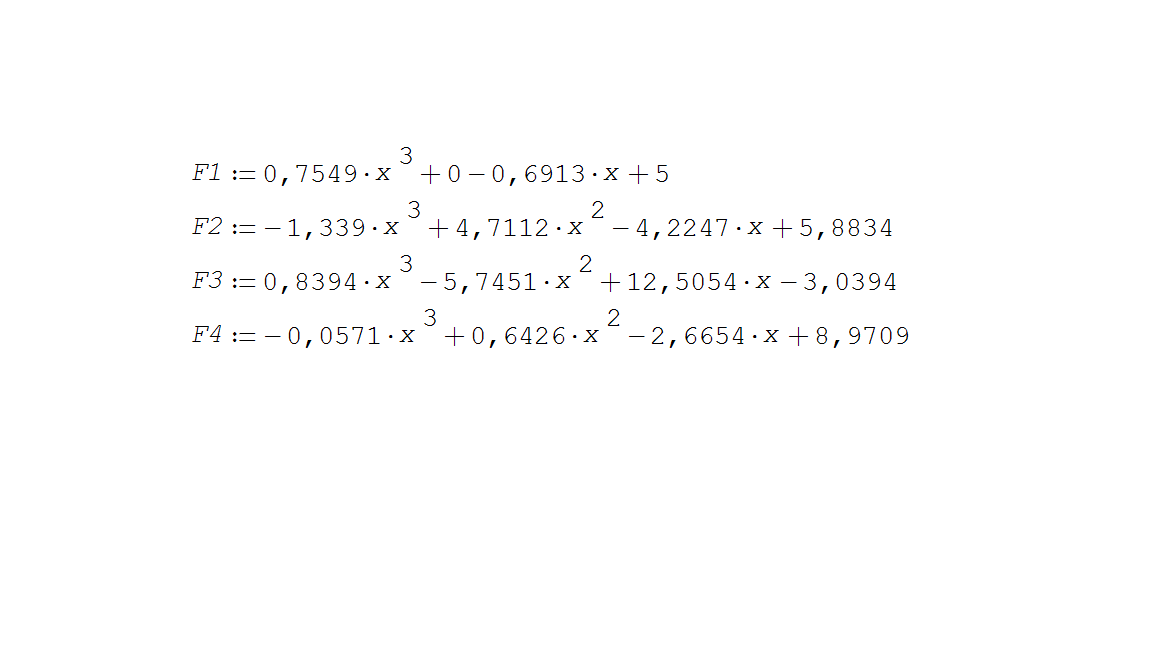
\includegraphics[scale=0.5]{16.png}\end{center}

\newpage
\begin{center}

{\bf Оценка погрешности интерполяции эрмитовыми
кубическими сплайнами}

\end{center}
Для нахождения погрешности нам нужно получить четвертую производную функции и подставить ее в формулу:
\\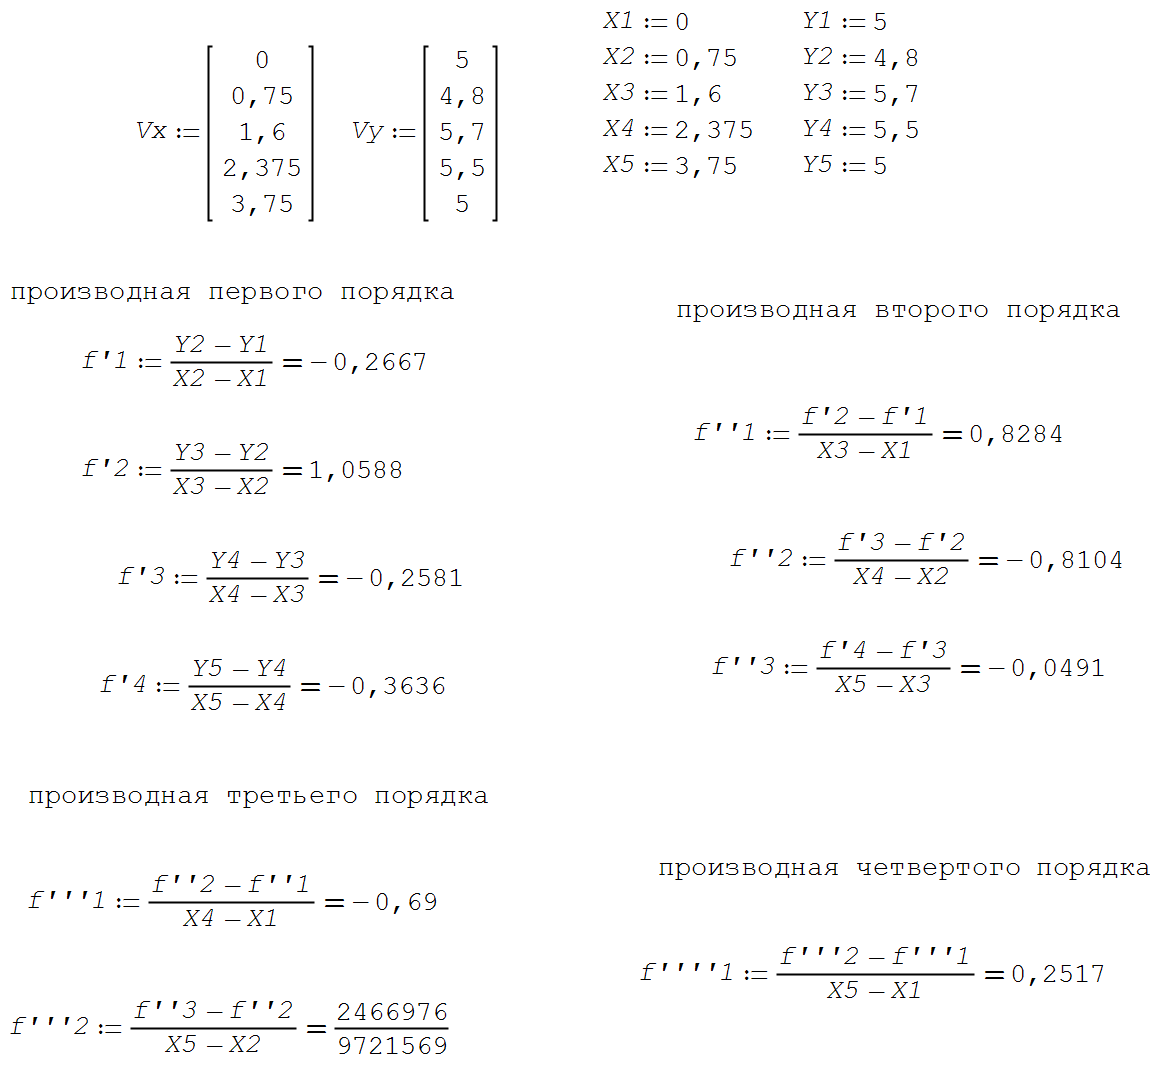
\includegraphics[scale=0.55]{18.png}
\\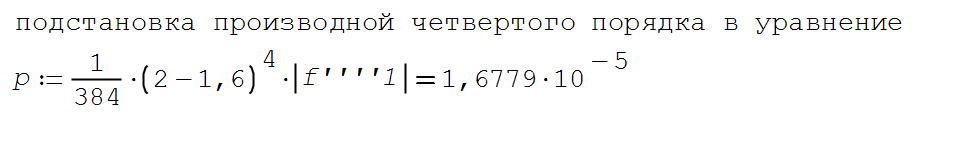
\includegraphics[scale=0.55]{19.png}
\newpage
\begin{center}{\bf построение кубического сплайна.}\\\end{center}

\begin{tikzpicture}

\begin{scope}[scale=2]


\draw[thin, ->] (0,0) -- (7,0) node[right] {$X$};
\draw[thin, ->] (0,0) -- (0,7) node[left] {$Y$};

\foreach \x\xtext in {0,1,2,3,4} 
\draw (\x,0.1) -- (\x,-0.1) node[below] {$\xtext$};
\foreach \y\ytext in {1,2,3,4,5,6} 
\draw (0.1,\y) -- (-0.1,\y) node[left] {$\ytext$};


\draw[domain=0:0.75, smooth, blue] plot ({\x},{(0.7549*(\x)*(\x)*(\x))+0-(0.6913*(\x))+5});
\draw[domain=0.75:1.6, smooth, red] plot ({\x},{(-1.339*(\x)*(\x)*(\x))+(4.7112*(\x)*(\x))-(4.2247*(\x))+5.8834});
\draw[domain=1.6:2.375, smooth,green] plot ({\x},{(0.8394*(\x)*(\x)*(\x))-(5.7451*(\x)*(\x))+(12.5054*(\x))-3.0394});
\draw[domain=2.375:3.75, smooth, violet] plot ({\x},{(-0.0571*(\x)*(\x)*(\x))+(0.6426*(\x)*(\x))-(2.6654*(\x))+8.9709});



\draw(0,5) circle (0.7pt);
\draw (0.75,4.8) circle (0.7pt);
\draw (1.6,5.7) circle (0.7pt);
\draw (2.375,5.5) circle (0.7pt);
\draw (3.75,5) circle (0.7pt);

\draw[thin,dashed] (0.75,4.8) -- (0.75,0);

\draw[thin,dashed] (1.6,5.7)  -- (1.6,0) ;

\draw[thin,dashed]  (2.375,5.4) --  (2.375,0);

\draw[thin,dashed] (3.75,5) -- (3.75,0);

\end{scope};
\end{tikzpicture}

$V_{x}=[0,0.75,1.6,2.375,3.75]$
$V_{y}=[5,4.8,5.7,5.5,5]$\\
Погрешность в точке Х=2.4 не превышает 0.0000016779\\
Значение в точке x=1.4 : 5.525 
\newpage
\begin{equation}\label{6}
\end{equation}
{\bf6. Задача оптимального распределения неоднородных ресурсов.}\\
Требуется решить следующую задачу оптимального распределения неоднородных ресурсов. Пусть в распоряжении завода железобетонных изделий (ЖБИ) имеется m видов сырья (песок, щебень, цемент) в объемах ${\bf a_i}$  .Требуется произвести продукцию {\bf n} видов. Дана технологическая норма $c_ij$  требления отдельного i-го вида сырь для изготовления единицы продукции каждого j-го вида. Известна прибыль $\pi_j$  получаема от выпуска единицы продукции j-го вида. Требуется определить, какую продукцию и в каком количестве должен производить завод ЖБИ, чтобы получить максимальную прибыль.\\
Исходные данные:\\
\begin{figure}[H]
\begin{center}
\begin{minipage}[h]{0.65\linewidth}
\center{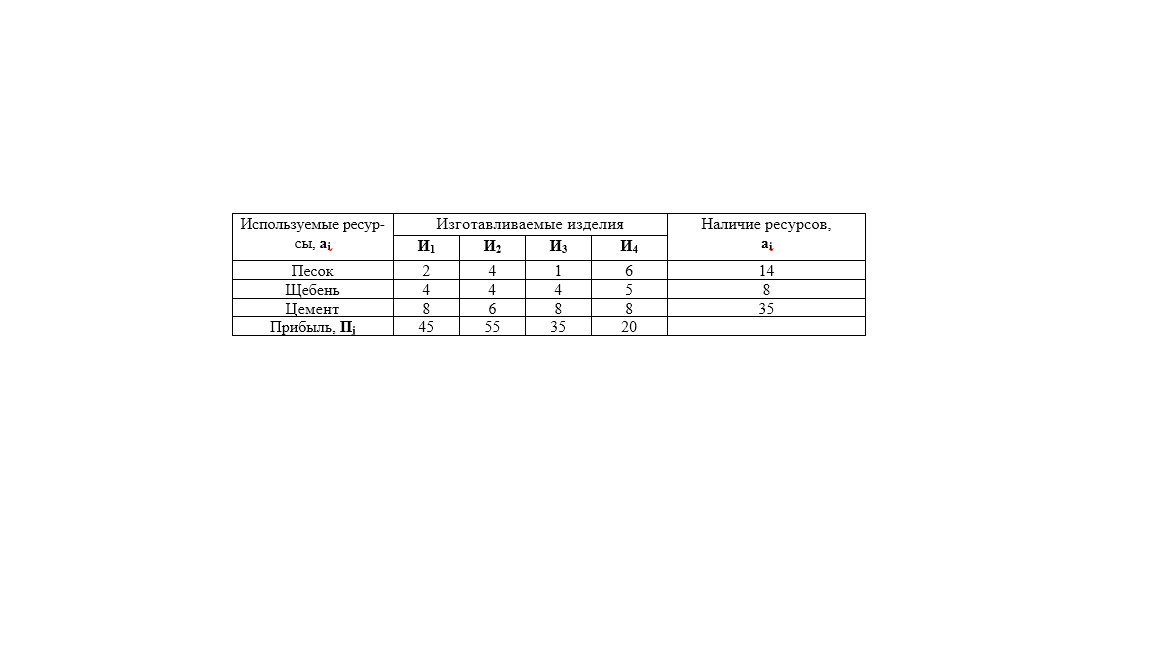
\includegraphics[width=1\linewidth]{1.png}}  \\
\end{minipage}
\end{center}
\end{figure}
Так как данная задача является целочисленной задачей линейного программирования (ILP), стандартная функция мат. пакета «SciLab» для решения задач линейного программирования karmarkar не даст верного решения, если оптимальное решение для соответствующей задачи без целочисленного ограничения не является целочисленным или «близким» к нему.

Для решения задачи воспользуемся средой программирования pascalABC.net 

Листинг кода:

program task_3;\\
var i1, i2, i3, i4: array [1..4] of integer;\\
	k1, k2, k3, k4, max, i, j, t, m, f:integer;\\
begin\\

	max := 0;\\
	
	i1[1] := 2;\\
	
	i1[2] := 4;\\
	
	i1[3] := 8;\\
	
	i1[4] := 45;\\
	
	i2[1] := 4;\\
	
	i2[2] := 4;\\
	
	i2[3] := 6;\\
	
	i2[4] := 55;\\
    
    i3[1] := 1;\\
	
	i3[2] := 4;\\
	
	i3[3] := 8;\\
	
    i3[4] := 35;\\
	
	i4[1] := 6;\\
	
	i4[2] := 5;\\
	
	i4[3] := 8;\\
	
	i4[4] := 20;\\
	
	t := 14;\\
	
	m := 8;\\
	
	f := 35;\\
	
	for i := 0 to 4 do\\
	
		for j := 0 to 4 do\\
		
		if (((t - i1[1]*j - i2[1]*j-i3[1]*j-i4[1]*j) >= 0) and ((m - i1[2]*i - i2[2]*j-i3[2]*j-i4[2]*j) >= 0) and ((f - i1[3]*i - i2[3]*j-i3[3]*j-i4[3]*j) >= 0)) then\\
		
		if ((i1[4]*i + i2[4]*j+i3[4]*j+i4[4]*j) > max) then\\
		
		begin\\
		
			max := i1[4]*i + i2[4]*j+i3[4]*j+i4[4]*j;\\
			
            k3 := k1;\\
            
            k4 := k2;\\
            
			k1 := i;\\
			
			k2 := j;\\
            
    
		end;\\
	write(max, ' ', k1, ' ', k2, ' ', k3, ' ', k4);\\
end.\\


Ответ программы:
90\ 2\ 0\ 1\ 0

Таким образом для достижения максимальной прибыли в 90 условных единиц предприятию необходимо произвести две единицs изделия №1 и одну единицу изделия №3.

\newpage
\begin{equation}\label{7}
\end{equation}
{\bf 7. Выводы}

Ознакомился с математическими пакетами "scilab" и "reduce". Научился применять полученные навыки при работе с ними. Полученные знания были использованы для решения задач: нахождения нулей функции, её аналитического исследования, интерполяции кубическими сплайнами функции от одной переменной, целочисленного линейного программирования.
\newpage
\begin{equation}\label{8}
\end{equation}
{\bf8. Список литературы}
\\1. Reduce. User’s manual
\\2. Introduction in SciLab
\\3. Optimization in SciLab
\\4.Ю.С. Завьялов. Методы сплайн-функций. М.Наука, 1980.
\\5.Introduction in SciLab
\\6.http://www.nsc.ru/win/docs/TeX/Tobias/lshort2e.html
\\7.http://lpsolve.sourceforge.net/5.1/Scilab.htm
\\8.smath studio user’s manual
\\9.pascalABC.net user’s manual
\end {document}